\section{Introducci\'on te\'orica}

El problema de Demosaicing consta de poder construir una imagen con información de los 3 canales en cada uno de sus pixel en base a una que sólo tiene definidos los valores de un sólo canal para cada celda. Este desafío es muy común en las camáras de fotos digitales ya que en realidad cada fotosensor detecta un sólo color, por lo cual a la imagen capturada hay que aplicarle algún procedimiento lógico para que el usuario final pueda verla efectivamente con todos los colores.

Particularmente estaremos analizando 4 algoritmos distintos que intentan solucionar esto. Ellos son: Vecinos, Bilineal, Direccional y High Quality. Todos estos deben aplicarse sobre imágenes en formato Bayer array, es decir, imágenes que en cada pixel tienen información sólo de un canal (Verde, Rojo o Azul) y estos además tienen una distribución especial (en la que por ejemplo el verde predomina en cantidad ya que es el color que mejor recepción tiene en el ojo humano).

\begin{figure}[htb]
\begin{center}
       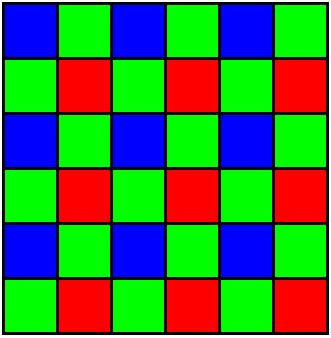
\includegraphics[width=0.2\textwidth]{imagenes/bayer.jpg}
       \caption{Patrón de píxeles en una imagen bayerizada}
       \end{center}

\end{figure}


Para nuestras pruebas lo que haremos es tomar imágenes con todos sus canales completos en todos lo pixeles y pasarlas al formato Bayer array. Como en lo que queremos hacer foco en este trabajo es la calidad de estos procedimientos y sus resultados, no nos interesa que la imagen Bayer haya sido tomada realmente por una cámara, es más, nos sirve más tener una imagen full color y transformala ya que así podemos comparar nuestros resultados contra la original.

Por esto es que desarrollamos una función muy simple que realiza esta transformación. Básicamente lo que hace es: 
\begin{itemize}
\item Celdas en columnas y filas pares, deja sólo el canal azul
\item Celdas en columnas y filas impares, deja sólo el canal rojo
\item En todas las otras dejamos sólo el canal verde
\end{itemize}   


\begin{figure}[h]
       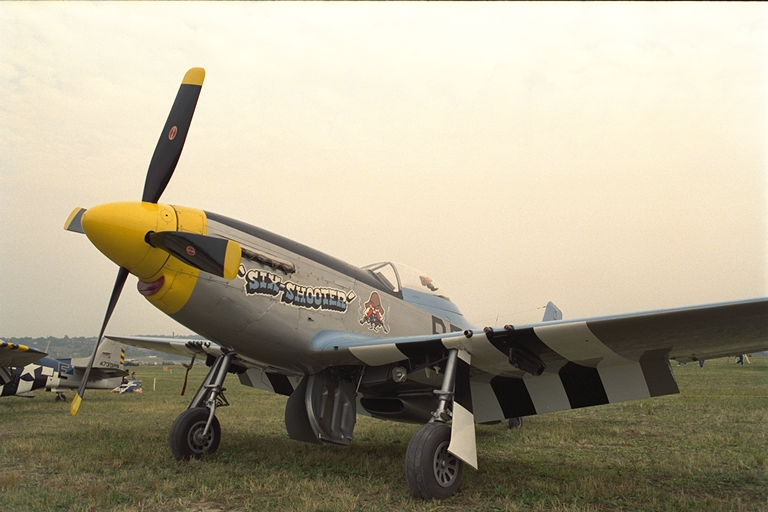
\includegraphics[width=0.5\textwidth]{imagenes/img9.png}
           \hfill
        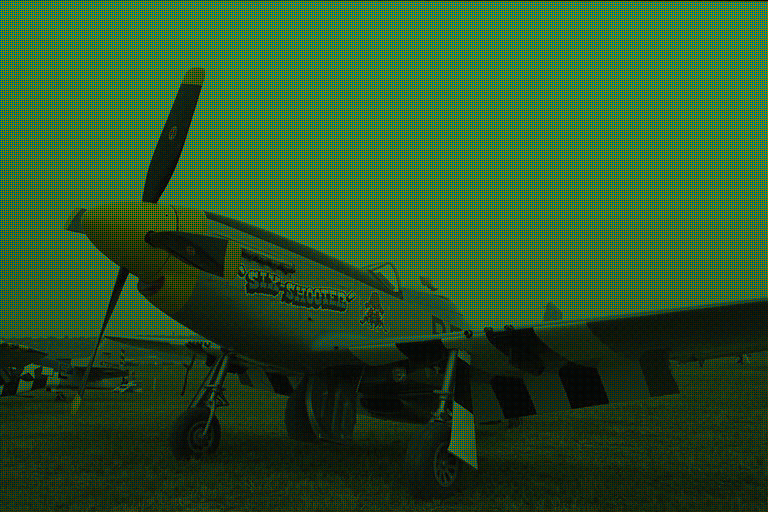
\includegraphics[width=0.5\textwidth]{imagenes/img9_bayer.png}   
        Imagen original y bayerizada
\end{figure}
\newpage
\subsection{Artifacts}

Una forma que utilizaremos para medir la calidad subjetiva de los distintos algoritmos de demosaicing para las imágenes con las que experimentaremos es mediante la detección de \textbf{artifacts}. Los artifacts son defectos comunes que ocurren en el procesamiento de imágenes y que han sido categorizados para un mejor análisis, entre los cuales podemos encontrar y nos enfocaremos: Moiré, False Color, Zippering, Blur y Ringing/Edge. Por tal motivo vamos a definir y mostrar un ejemplo de cada uno:

\paragraph{Moiré:}
El artifact Moiré ocurre en zonas de la imagen en donde hay lineas muy cercanas y que producto de los algoritmos de demosaicing se producen superposiciones de las mismas, dando como resultado en la mayoría de los casos un nuevo patrón sobre ellas

\begin{figure}[htb]
\begin{center}
       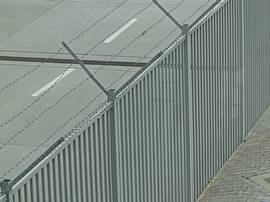
\includegraphics[width=0.4\textwidth]{imagenes/moire_original.jpg}
          \hfill
           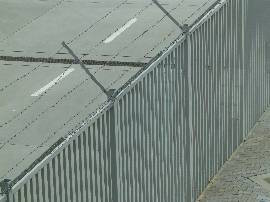
\includegraphics[width=0.4\textwidth]{imagenes/moire_example.jpg}
          
       Ejemplo de imagen original vs artifact Moiré
       \end{center}

\end{figure}

\paragraph{False Color:}
El artifact False Color ocurre cuando el algoritmo de demosaicing arroja como resultado una zona en la imagen de distinto color al original. Suele venir acompañado cuando ocurre Moiré

\paragraph{Zippering:}
El artifact Zippering (cremallera) es un artifact que suele ocurrir en zonas de la imagen donde hay elementos borde, donde en la misma se genera un cambio abrupto en los valores, y consiste en que se produce un efecto de lineas que tienen mucha similitud a una cremallera en estos bordes

\begin{figure}[htb]
\begin{center}
       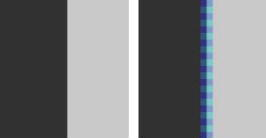
\includegraphics[width=0.5\textwidth]{imagenes/zippering_example.jpeg}
       \caption{Ejemplo de imagen original vs artifact Zippering}
       \end{center}

\end{figure}
\paragraph{Blur:}
Como su nombre lo indica, el artifact Blur (borroneo) se observa cuando la imagen se ve más borrosa, con menos nitidez y definición que la original

\begin{figure}[htb]
\begin{center}
       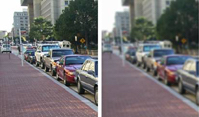
\includegraphics[width=0.5\textwidth]{imagenes/blur_example.jpg}
       \caption{Ejemplo de imagen original vs artifact Blur}
       \end{center}

\end{figure}


\paragraph{Ringing:}
El artifact Ringing aparece con frecuencia en zonas de borde  produciendo que los mismos pierdan suavidad (los bordes sufren un pixelamiento) y aparezca un \textit{borde fantasma}, que consiste en un borde alrededor como si fuese una sombra del mismo borde.

\begin{figure}[htb]
\begin{center}
       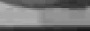
\includegraphics[width=0.5\textwidth]{imagenes/ringing_example.jpg}
       \caption{Ejemplo de artifact Ringing en borde recto y redondeado}
       \end{center}

\end{figure}

